\documentclass{beamer}
\usepackage{minted}
\usepackage{graphicx}
\usepackage[utf8]{inputenc}
\usepackage{longtable, multicol}

\setbeamertemplate{navigation symbols}{}

\title{\LaTeX}

\subtitle{lay-teck}

\author{Some Guy}
\institute{Linux@APP}
\date{02/21/2018}
 
\begin{document}

\frame{\titlepage}
\begin{frame}
\frametitle{What is \LaTeX?}
LaTeX is a typesetting system, desgned to prevent the document writer from screwing everything up.
Latex is acutaly a collection of macros built ontop of TeX to make it useable for document writers, LaTeX. Instead of visually formatting your text, you enter your document text intertwined with LaTeX commands in a text file. You then run TeX to produce formatted output, such as a PDF file. Thus, in contrast to standard word processors, your document is a separate file that does not pretend to be a representation of the final typeset output, and so can be easily edited and manipulated. 

\end{frame}
% types of documents
\begin{frame}[fragile]
\frametitle{Types of documents.}
\renewcommand*{\arraystretch}{1.4}
\begin{longtable}{l p{3 in}}
article: &     For articles in scientific journals, presentations, short reports, program documentation, invitations, ... \\
IEEEtran: &    For articles with the IEEE Transactions format. \\
proc: &        A class for proceedings based on the article class. \\
report: &      For longer reports containing several chapters, small books, thesis. \\
book: &        For real books. \\
slides: &      For slides. The class uses big sans serif letters. \\
memoir: &      For changing sensibly the output of the document. It is based on the book class, but you can create any kind of document with it. \\
letter: &      For writing letters. \\
beamer: &      For writing presentations. \\
\end{longtable}
\end{frame}

\begin{frame}[fragile]
\frametitle{A frame}
Framy stuff.

{\LaTeX} or \verb|\LaTeX|
\begin{multicols}{2}
\begin{verbatim}
\documentclass{article}
\title{A paper on how to
write papers.}
\date{2018-02-22}
\author{Andrew Pobrica}
\begin{document}

\maketitle
\pagenumbering{gobble}
\newpage
\pagenumbering{arabic}

\section{Section}
Hello World!
\subsection{Subsection}
Stucturing a document is easy!
\subsubsection{Subsubsection}
More text.
\paragraph{Paragraph}
Some more text.
\subparagraph{Subparagraph}
    Even more text.
\section{Another section}
\end{document}
\end{verbatim}
\end{multicols}
\end{frame}

% Python3 code
\begin{frame}[fragile]

% must install pygments for minted to work can be 2 or 3
% run latex compiler with -shell-escape as well
\begin{minted}{python3}

#Leibniz formula

pi = 0
x = 0
iterations = 10000
try:
        for x in range(iterations):
                pi = pi + 2 / ((4*x+1) * (4*x+3))
        print(pi*4)

except KeyboardInterrupt:
        print(x)
        print(pi*4)


\end{minted}

\end{frame}

\begin{frame}
tlmgr update --list

tlmgr update --self

tlmgr update --all

tlmgr uninstall
\begin{figure}{Fig. 1: I got this off of reddit.}
\centering
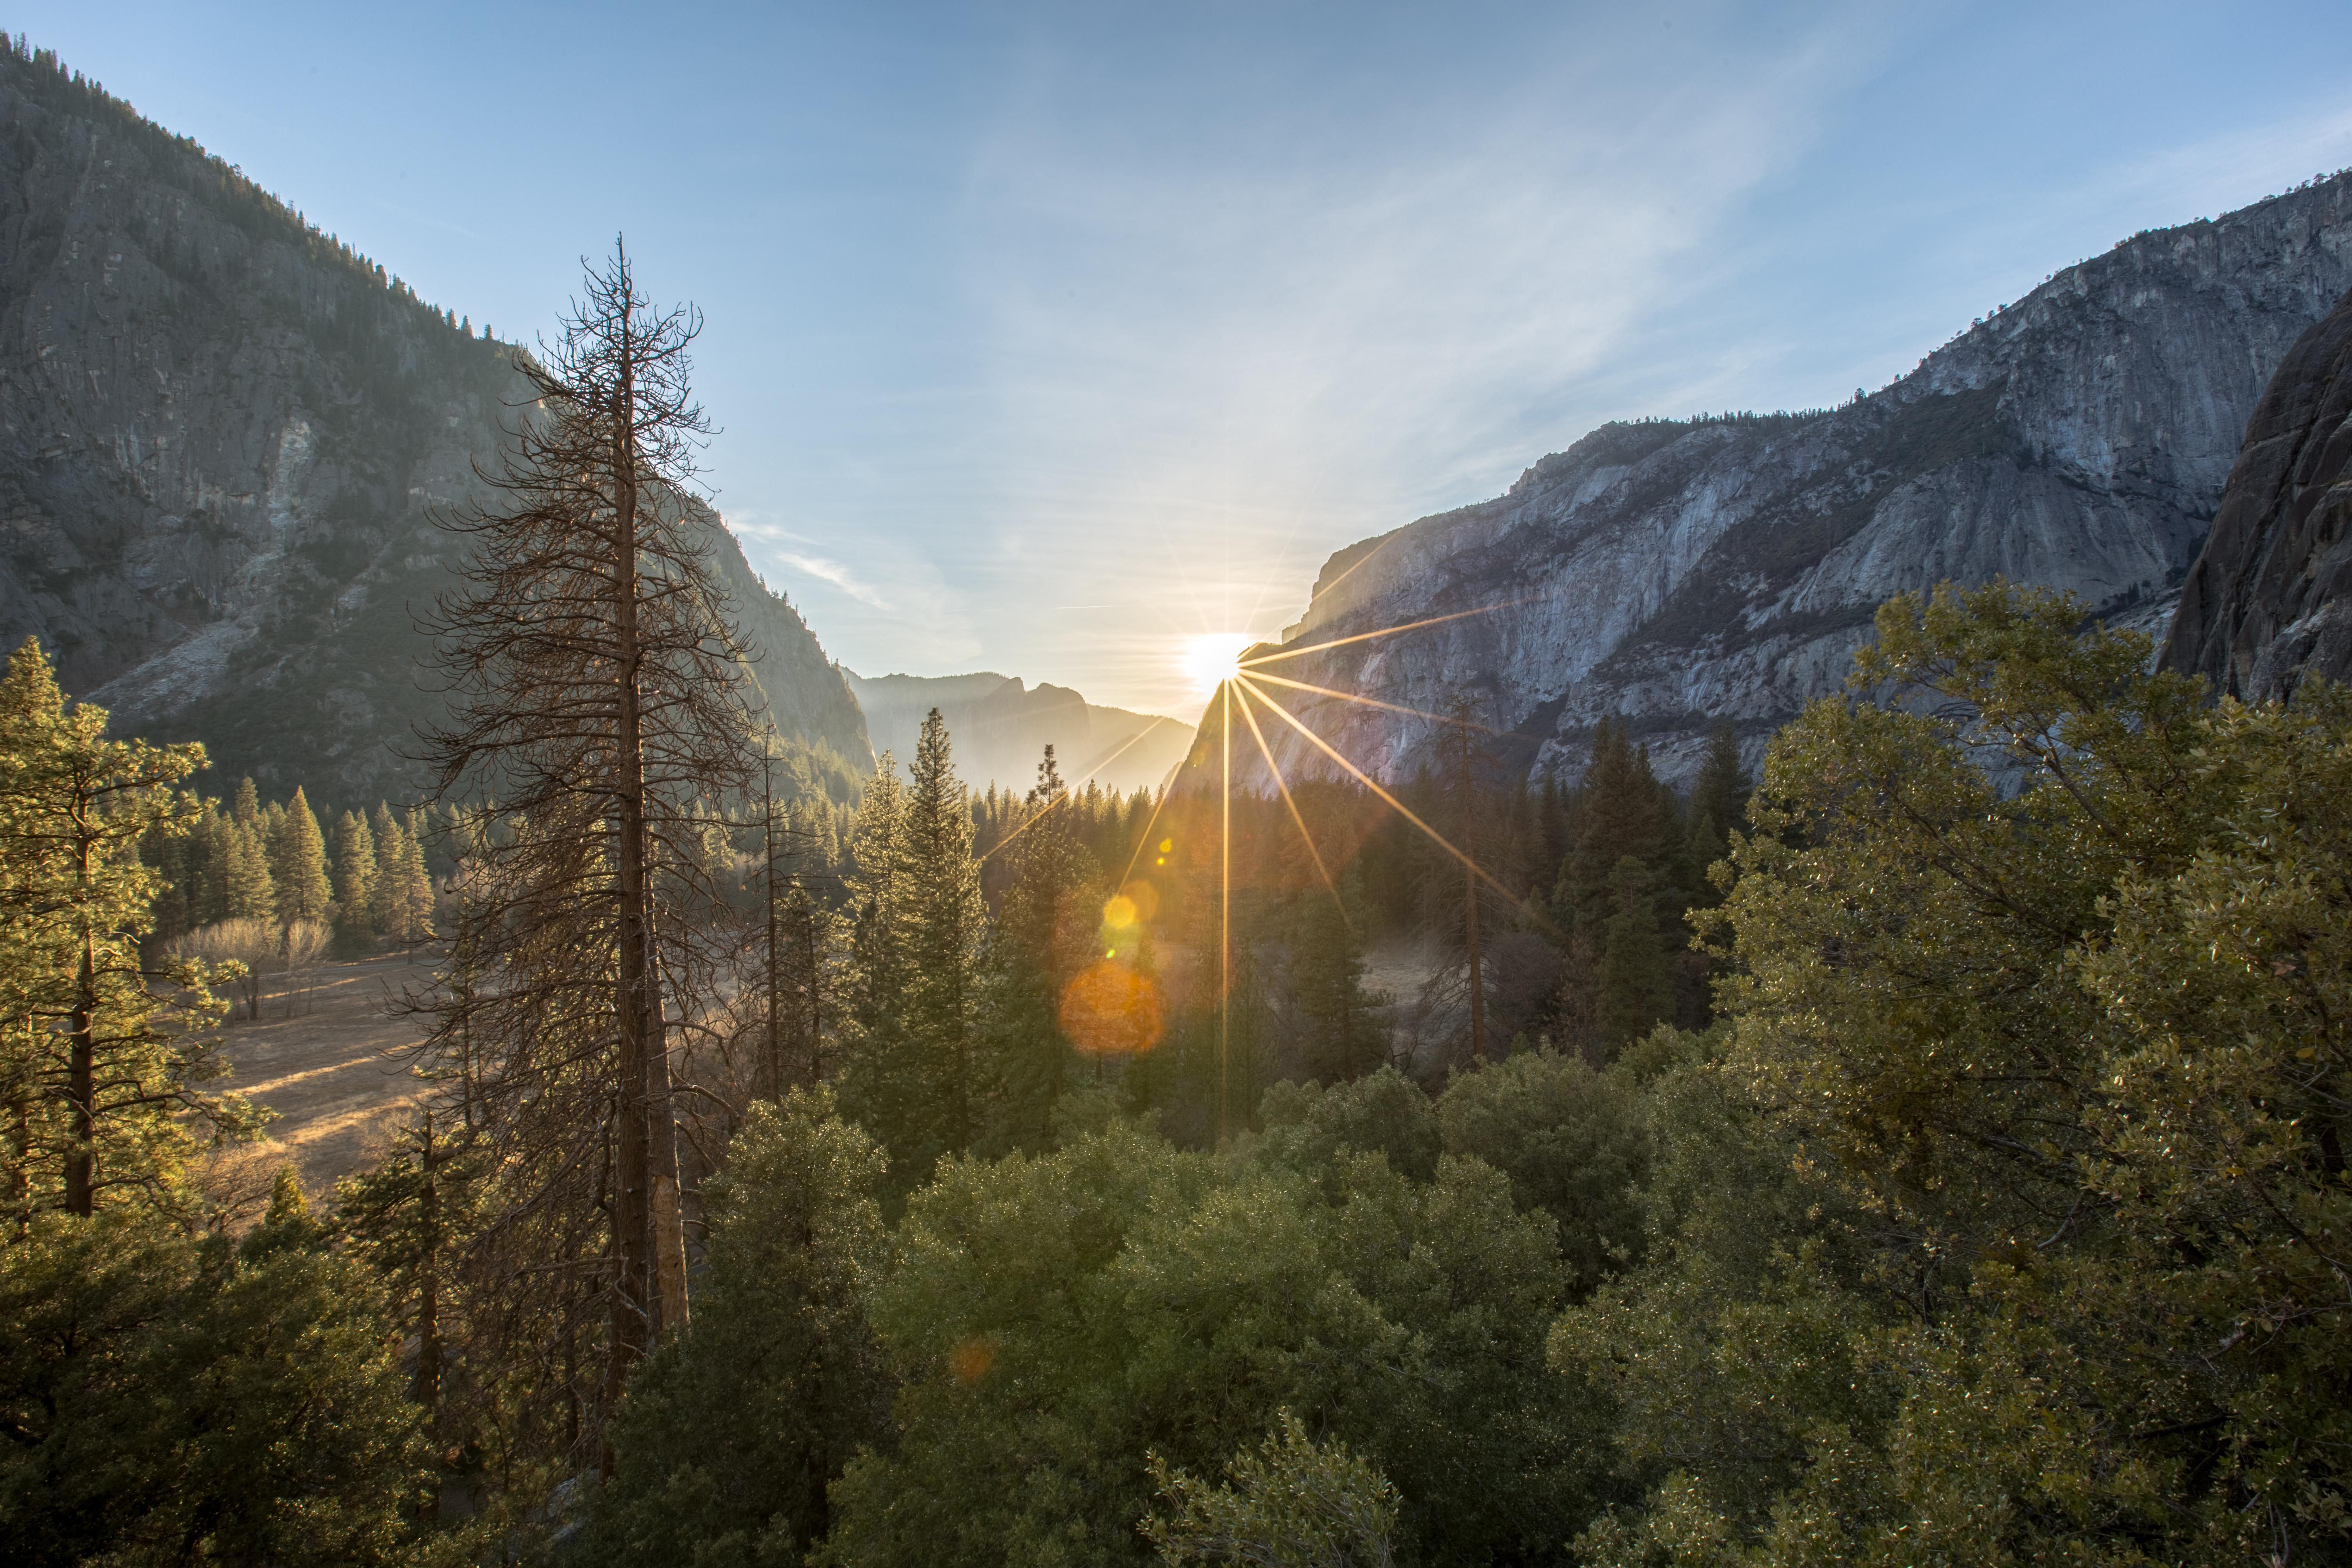
\includegraphics[height=2.5in]{picture1}
\end{figure}
\end{frame}

% bash stuff
\begin{frame}[fragile]
% must install pygments for minted to work can be 2 or 3
% run latex compiler with -shell-escape as well
\input{cowsay}
\end{frame}

\begin{frame}[fragile]
\begin{minted}{latex}
\LaTeX
\end{minted}
\end{frame}

\end{document}
